\documentclass[a4paper,12pt]{book}
\usepackage{graphicx}
\usepackage[export]{adjustbox}
\usepackage{subcaption}
\graphicspath{{Pics/}}
\usepackage{charter}
\usepackage{fancyhdr}
\usepackage{enumerate}
\usepackage{enumitem}
\usepackage{siunitx}
\usepackage{amssymb}
\usepackage{longtable}
\usepackage{multicol}
\usepackage{multirow}
\usepackage{hhline}
\usepackage{parskip}
\setlength{\parskip}{6pt}
\usepackage{ragged2e}
\usepackage{geometry} %margin
\geometry{left=2.1cm,right=2.1cm,top=3cm,bottom=3cm}
\usepackage{setspace}
\SetSinglespace{1.2}
\singlespacing
\renewcommand{\ttfamily}{\fontfamily{pcr}\selectfont}
%\renewcommand{\familydefault}{\rmdefault}

\usepackage[,table]{xcolor}
\definecolor{LightBlue}{cmyk}{0.16,0.03,0.04,0}
\definecolor{Title}{cmyk}{0.8,0.1,0,0.3}
\setlength{\arrayrulewidth}{0.3mm}
\setlength{\tabcolsep}{2pt}
\setlength{\headheight}{15pt}
\renewcommand{\arraystretch}{1}
\usepackage{tikz}
\usepackage{nicematrix}
\newcommand*\circled[1]{\tikz[baseline=(char.base)]{\node[shape=circle,draw,inner sep=1pt] (char) {#1};}}

\newcolumntype{s}{>{\columncolor{Title}\RaggedLeft} m{3.5em}} % columntype for chapter title
\newcolumntype{d}{>{\columncolor{LightBlue}\RaggedRight} m{\textwidth}} % columntype for code bloc
\newcolumntype{a}{>{\columncolor{LightBlue}\RaggedRight} m{0.96\textwidth}} % columntype for secondary code bloc

\usepackage{titlesec}
\usepackage[hidelinks]{hyperref}
\urlstyle{same}

\captionsetup[figure]{labelsep=period,font={bf}}
\captionsetup[table]{font={bf},labelsep=period}

\newcommand{\titlename}{}

\newcommand{\chaptertitle}[2]{ %reset chapter format
\vspace{-120pt}
\gdef\titlename{#1}
{
\SetSinglespace{1.1}
\singlespacing
\Huge\bfseries
\setlength{\tabcolsep}{8pt}
\renewcommand{\arraystretch}{1.5}
\begin{tabular}{s >{\RaggedRight}m{14.5em}}
\textcolor{white}{Chapter\newline\thechapter}&\textcolor{Title}{#2}
\end{tabular}
}
}

\newcommand{\partpic}[1]{%insert picture
    \tikz[remember picture,overlay] \node at (current page.center){\includegraphics[width=\paperwidth]{#1}};
}

\titleformat{\part} %reset part %format
{\huge\bfseries} % format
{} % label
{0em} % sep
{\Centering} % before-code

\titleformat{\chapter} %reset chapter %format
{\huge\bfseries} % format
{} % label
{0em} % sep
{\Centering} % before-code
\titlespacing{\chapter}{0pt}{0pt}{0pt}

\titleformat{\section} %reset section %format
{\Large\bfseries} % format
{\textcolor{Title}{\thesection}} % label
{0.5em} % sep
{\color{Title}} % before-code
\titlespacing{\section}{0pt}{12pt}{6pt}

\titleformat{\subsection} %reset subsection %format
{\large\bfseries} % format
{\textcolor{Title}{\thesubsection}} % label
{0.5em} % sep
{\color{Title}} % before-code
\titlespacing{\subsection}{0pt}{8pt}{6pt}

\newenvironment{term}[1]{
    \textbf{#1}

    \leftskip 1em
    \parskip 0pt
}

\newenvironment{secterm}[1]{
    \textbf{#1}

    \leftskip 2em
    \parskip 0pt
}

\newenvironment{codebloc}{ %define code bloc style
    \ttfamily\footnotesize
    \renewcommand{\arraystretch}{1}
}

\newcommand{\note}[2][NOTE]{ %Note/Tips
\vspace{6pt}
\begin{tabular}{b{\textwidth}}
\hline
\fontfamily{phv}\selectfont \textbf{#1}\\
\leftskip 1em #2\\
\hline
\end{tabular}
}

\newcommand{\secnote}[2][NOTE]{ %Note/Tips
\vspace{6pt}
\begin{tabular}{b{0.93\textwidth}}
\hline
\fontfamily{phv}\selectfont \textbf{#1}\\
\leftskip 1em #2\\
\hline
\end{tabular}
}

\title{ESP32-C3 Wireless Adventure\par \Large A comprehensive guide to IoT}
\author{Espressif Systems}
\date{\today}

\pagestyle{fancy} % reset head&foot
\fancyhead{} % clear all header fields
\renewcommand\headrulewidth{0pt}
\fancyfoot{} % clear all footer fields
\setcounter{chapter}{10}

\begin{document}

\fancyfoot[LE]{\fontfamily{cmss}\selectfont{\textbf{\thepage} \ \textit{ESP32-C3 Wireless Adventure: A comprehensive guide to IoT}}}
\fancyfoot[RO]{\fontfamily{cmss}\selectfont{\textit{Chapter \thechapter. \titlename} \ \textbf{\thepage}}}

\chapter[Firmware Upgrade and Version Management]{\chaptertitle{Firmware Upgrade and Version Management}{Firmware Upgrade and\newline Version Management}}

\vspace{36pt}
The firmware update of IoT devices is often implemented through OTA (Over-the-Air). OTA provides a secure and dependable means to remediate firmware vulnerabilities, introduce novel functions, and optimize product performance, thereby enhancing the experience of end users. At present, OTA has become a standard function in the mass production of products.

Marking firmware with different versions based on their respective functionalities is a reliable and effective means of firmware management. Standardized methods of version marking can facilitate version management, aid in troubleshooting, and enable efficient post-upgrade tracking, ultimately leading to more effective firmware updates via OTA.

ESP-IDF provides an example of OTA and various firmware version management methods. This chapter will cover these topics and demonstrate how to achieve remote OTA for an intelligent lamp using ESP RainMaker.

\section{Firmware Upgrade}
The OTA mechanism allows the device to receive new firmware during normal operation, and write the new firmware to the currently inactive application partition. After verifying the validity of the firmware, the device switches to run on the new firmware. The basic steps of OTA are shown in Figure 11.1.

\begin{figure}[!h]
    \centering
    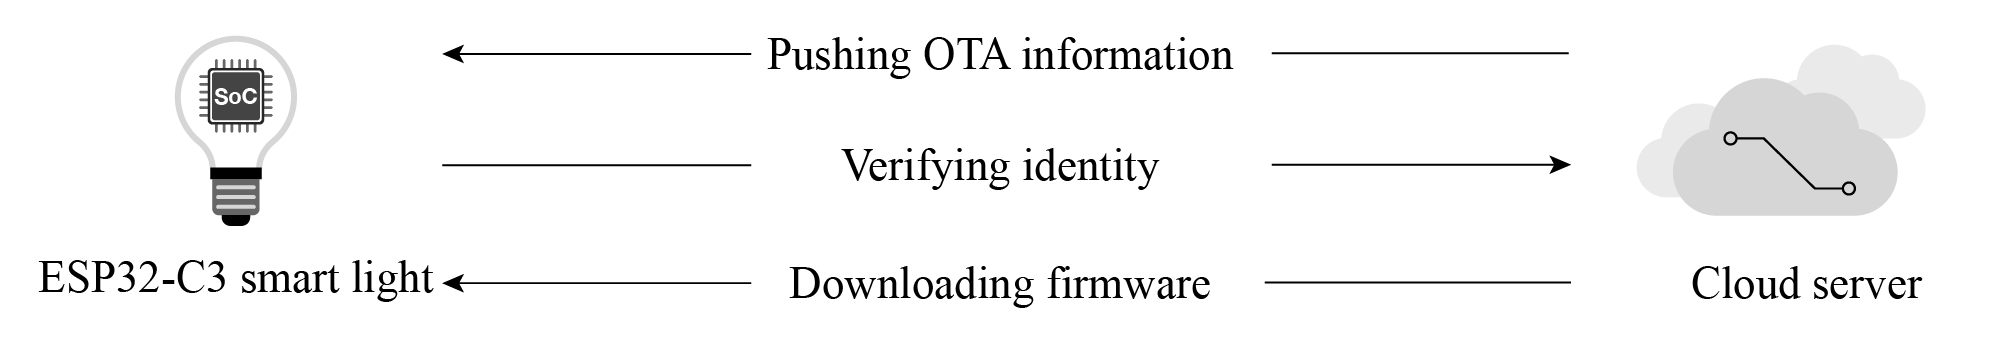
\includegraphics[width=0.7\textwidth]{D11Z/11-1}
    \caption{Basic steps of OTA}
\end{figure}

From Figure 11.1, the basic steps of OTA are as follows:

\begin{enumerate}[label=(\arabic*)]
    \item The cloud server pushes OTA information to the device.
    \item The device verifies the identity of the cloud server and downloads the firmware from the trusted cloud server.
    \item The device decides whether to perform OTA according to the version information in the firmware. If it decides to perform OTA, the firmware is then requested and written to the flash. After the verification is successfully completed, the system switches to run on the new firmware.
\end{enumerate}

According to the basic steps listed above, to put it simply, the OTA process is the process of firmware acquisition, writing, verification, and switching. Before further understanding the OTA mechanism, we will first introduce the partition table and firmware startup process.

\subsection{Overview of Partition Tables}
The partition tables in ESP-IDF refer to the descriptive files that divide the flash into specific functional areas at the user level. This book takes \href{https://github.com/espressif/esp-idf/tree/master/examples/system/ota/advanced_https_ota}{\texttt{advanced\_https\_ota}} as an example, abbreviated as the OTA upgrade example. In this example, the \href{https://github.com/espressif/esp-idf/blob/master/components/partition_table/partitions_two_ota.csv}{\texttt{partitions\_two\_ota.csv}} file under the \verb|partition_table| component in ESP-IDF is used by default. The following is a summary of the \verb|partitions_two_ota.csv| partition table.

\begin{codebloc}
\begin{tabular}{d}
\vspace{2pt}
\begin{verbatim}
1.  # Name,   Type, SubType, Offset,   Size, Flags
2.  # Note: if you have increased the bootloader size, make sure to update the 
offsets to avoid overlap
3.  nvs,        data,   nvs,        ,       0x4000,
4.  otadata,    data,   ota,        ,       0x2000,
5.  phy_init,   data,   phy,        ,       0x1000,
6.  factory,    app,    factory,    ,       1M,
7.  ota_0,      app,    ota_0,      ,       1M,
\end{verbatim}
\verb|8.  ota_1,      app,    ota_1,      ,       1M,|
\end{tabular}
\end{codebloc}

From the overview above, each entry in the partition table consists of \verb|Name|, \verb|Type|, \verb|SubType|, \verb|Offset|, \verb|Size|, and \verb|Flags|.

\begin{itemize}[leftmargin=1em]
    \item The \verb|Name| field is used to identify the name and should not exceed 16 bytes.
    \item The \verb|Type| field can be specified as either \verb|app| or \verb|data|, or a number from 0 to 254 (or the corresponding hexadecimal number 0x00 to 0xFE). It is mainly used to mark whether the stored content is an application firmware or data.
    \item The length of the \verb|SubType| field is 8 bits, and the specific marking content is related to the \verb|Type| field.
    \begin{itemize}[leftmargin=1em]
        \item[-] When \verb|Type| is defined as \verb|app|, \verb|SubType| can be specified as \verb|factory(0x00)|, \verb|ota_0|\\ \verb|(0x10)|, ..., \verb|ota_15(0x1F)|, or \verb|test(0x20)|.
        \item[-] When \verb|Type| is defined as \verb|data|, \verb|SubType| can be specified as \verb|ota(0x00)|, \verb|phy(0x01)|, \verb|nvs(0x02)|, \verb|nvs_keys(0x04)|, or a specific subtype for other components.
    \end{itemize}
    \item The \verb|Offset| and \verb|Size| fields are used to define a specific area.
    \item The \verb|Flags| field is used to mark whether encryption is enabled.
\end{itemize}

Without any value filled in the \verb|Offset| field, the partition table in the example is still valid. This is because the position of the first entry in the partition table is determined, so the address of the subsequent entry can be calculated from the \verb|Size| field of the previous entry. If the addresses of each entry in the partition table are not continuous, the \verb|Offset| field needs to be used to mark the starting address of each entry. For easy understanding, this book has converted the example partition table into a figure, as shown in Figure 11.2.

\begin{figure}[!h]
    \centering
    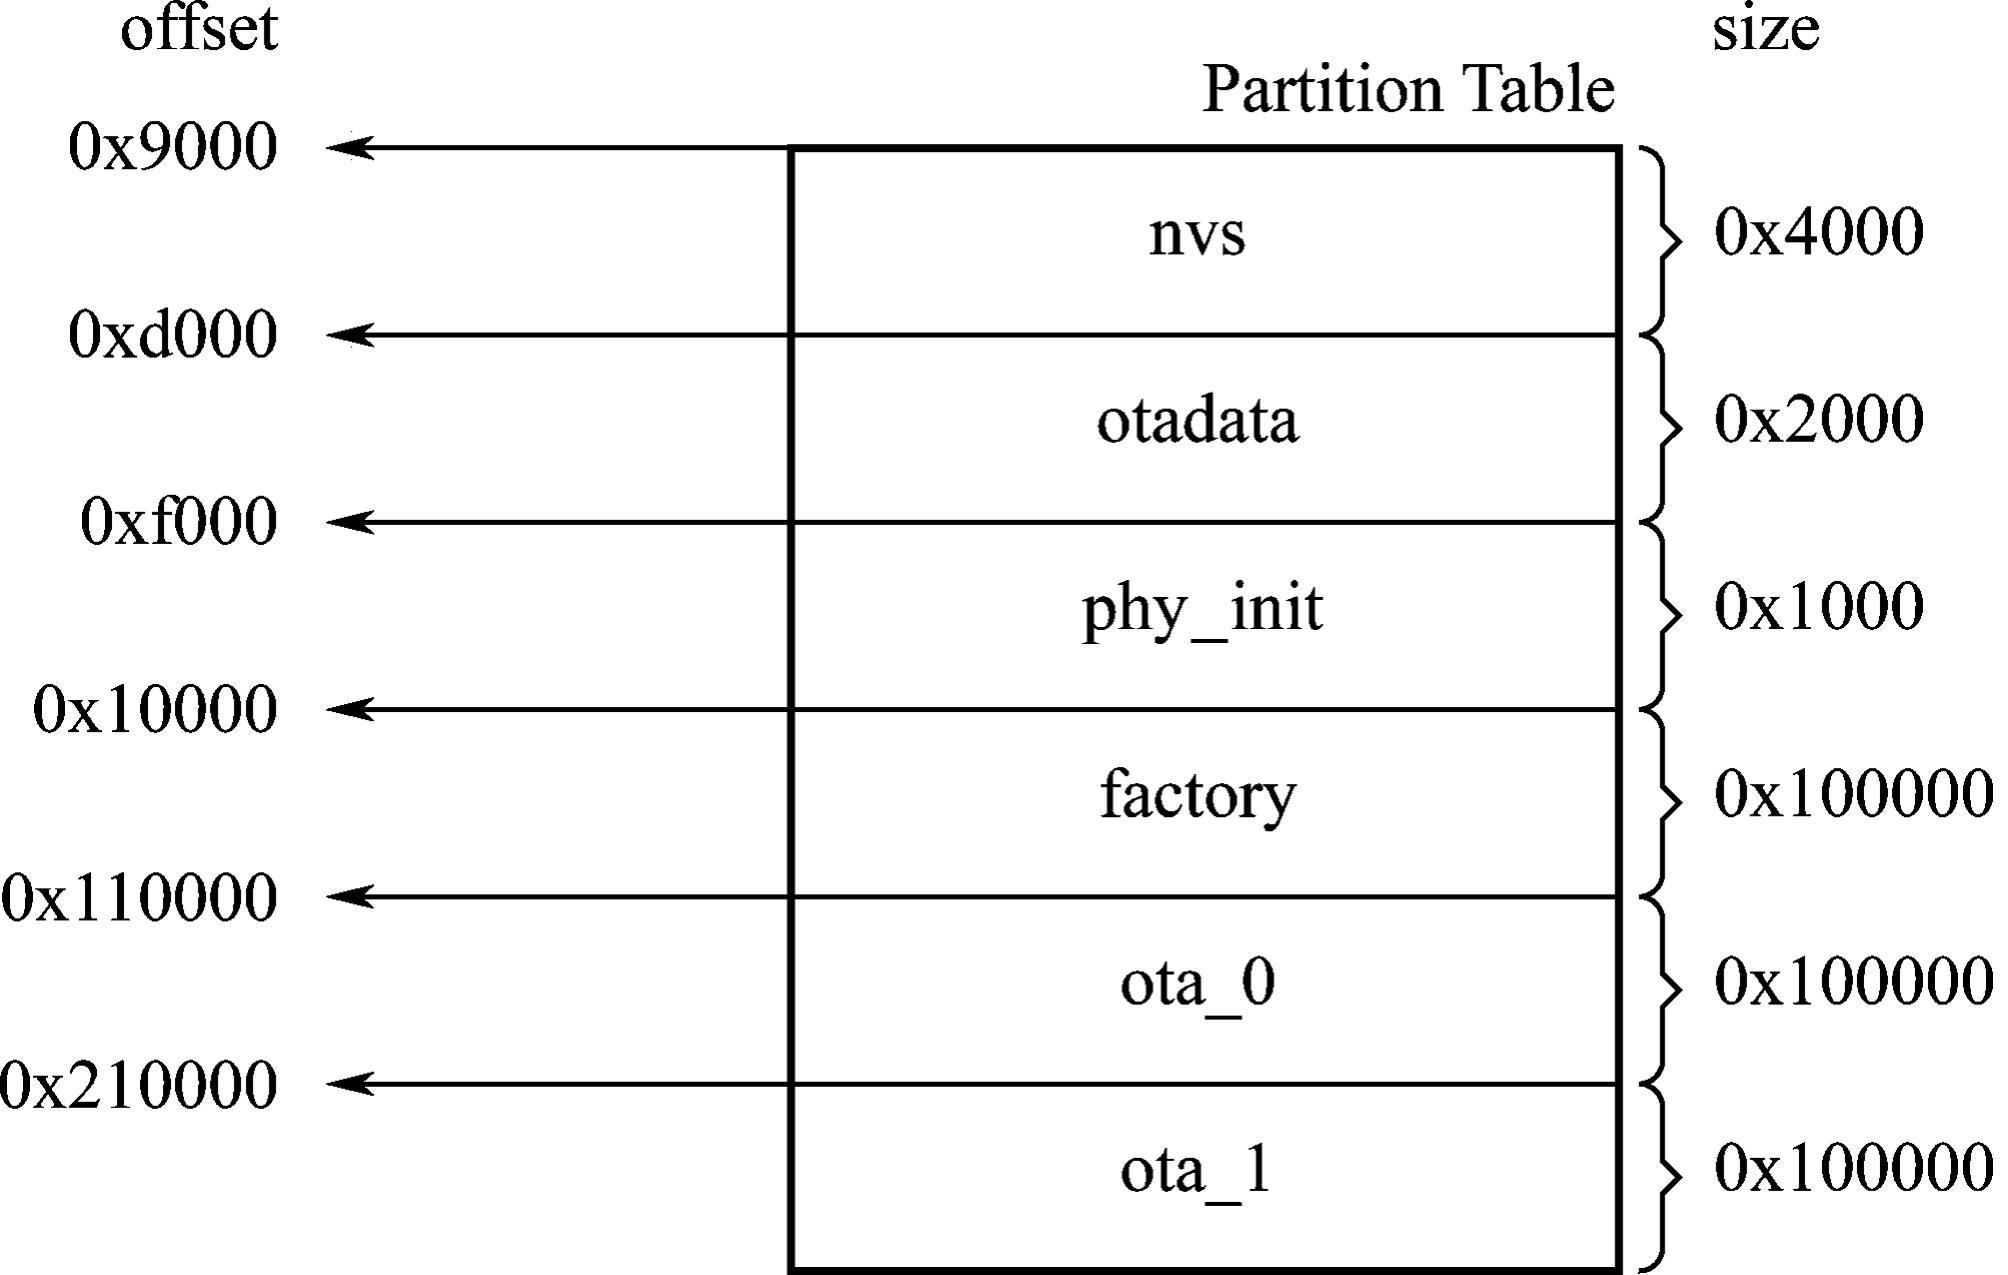
\includegraphics[width=0.7\textwidth]{D11Z/11-2}
    \caption{Schematics of the partition table}
\end{figure}

From Figure 11.2, the starting address of the first entry in the partition table is 0x9000, that is, the \verb|Offset| field of the entry whose \verb|Name| is \verb|nvs| in \verb|partitions_two_ota.csv| is 0x9000, and the size of this entry is 0x4000. According to the calculation rules introduced earlier, the \verb|Offset| of the next entry is 0x9000 + 0x4000 = 0xd000. Calculated sequentially, the \verb|Offset| of the last \verb|ota_1| entry should be 0x210000.

The \verb|partitions_two_ota.csv| partition table is divided into six areas: three data partitions \verb|nvs|, \verb|otadata|, and \verb|phy_init| are used to store NVS data, OTA data, and PHY initialisation data, respectively; and three application partitions used to store three different application firmwares. As can be seen from the basic steps of OTA, at least two OTA application partitions are required to perform OTA: \verb|[Type (app), SubType (ota_0/ota_1)]| and one OTA data partition \verb|[Type (data), SubType (ota)]|. It may also include an optional application partition, which is the factory application partition: \verb|[Type (app), |\\ \verb|SubType (factory)]|.

\begin{itemize}[leftmargin=1em]
    \item The OTA data partition is used to store information about the currently selected OTA application partition. After the first OTA, the OTA data partition will be updated to specify which OTA application partition to boot next. The size of the OTA data partition needs to be set to 0x2000 to prevent problems caused by power failure during writing. The two sectors are erased and written with matching data separately. If there is an inconsistency, the counter field will be used to determine the sector with the latest data.
    \item The application partition is used to store firmware. The factory application partition is the default application partition. If there is no OTA data partition or the OTA data partition is invalid, the firmware of the factory application partition (if it exists) will be used first, followed by the firmware of the OTA data partition. OTA will never update the contents of the factory application partition.
\end{itemize}

\subsection{Firmware Boot Process}
In Section 11.1.1, we introduced that the starting address of the first entry in the partition table is 0x9000. But why is the starting address not 0x0? And why is it 0x9000? To answer these questions, let's first look at Figure 11.3, which presents the specific contents stored in a 4 MB flash.

\begin{figure}[!h]
    \centering
    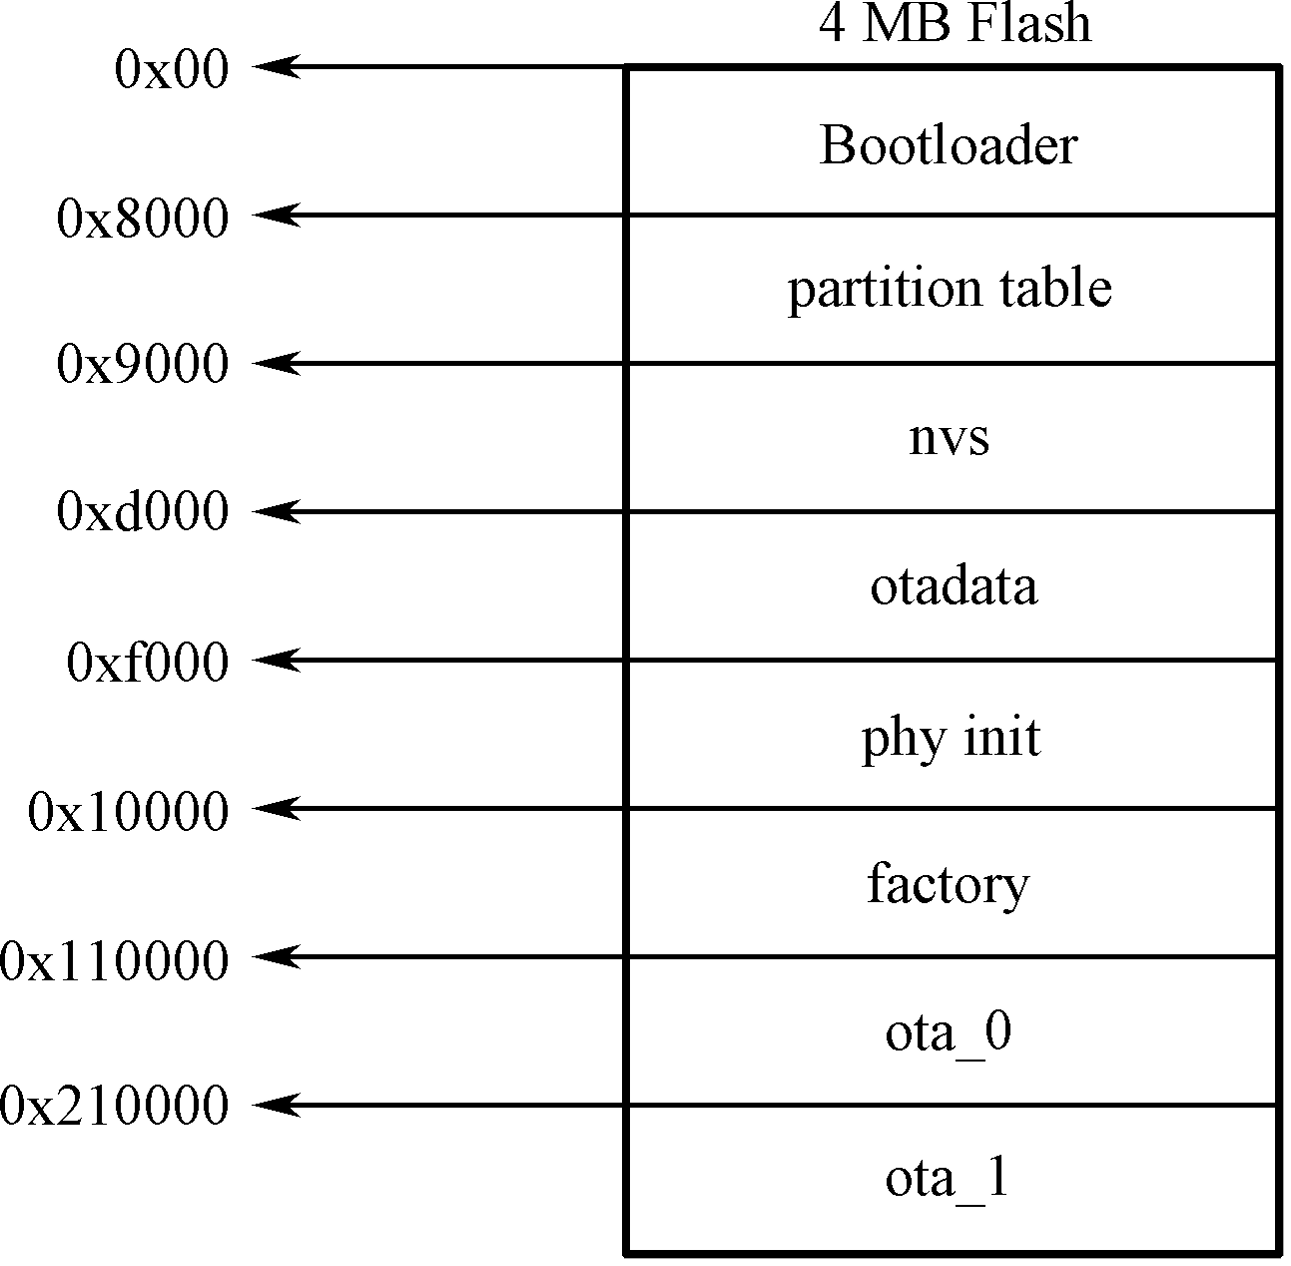
\includegraphics[width=0.5\textwidth]{D11Z/11-3}
    \caption{Specific contents stored in a 4 MB flash}
\end{figure}

As can be seen from Figure 11.3, the flash is divided into eight areas: the address 0x00 stores the Bootloader, the address 0x8000 stores the partition table, and the latter 6 areas, starting from 0x9000, is the area divided by the partition table, which you may already be quite familiar with. Now we can answer the first question. The reason why 0x0 is not the starting address is that it stores the Bootloader (not every 0x0 address of the chip flash stores the Bootloader. ESP32 series chips store the Bootloader at 0x1000), which is used to load and boot the application partition. In the programming design of Espressif chips, Bootloader is called the secondary bootloader, which mainly increases the flexibility of flash partition and facilitates the implementation of flash encryption, secure boot, and OTA functions. The secondary bootloader loads the partition table from the offset address of flash at 0x8000 by default. The size of the partition table is 0x1000. The secondary bootloader will look for the factory application partition and the OTA data partition from the partition table and determine which partition to boot by querying the OTA data partition. Therefore, the second question has also been answered.

The process from power-up to running the \verb|app_main()| function on ESP32-C3 can be divided into three steps:

\begin{enumerate}[label=(\arabic*)]
    \item Bootstrapping is performed by the primary bootloader, which is stored in the ROM of the ESP32-C3. Upon the chip reset, the CPU starts running immediately to determine the boot mode and perform relevant operations. The secondary bootloader is then loaded into RAM from the offset address 0x0 of the flash.
    \item Bootstrapping is performed by the secondary bootloader. The secondary bootloader will first load the partition table from flash and then query the OTA data partition to select a firmware from a particular application partition for loading. When all data is processed, the secondary bootloader will verify the integrity of the firmware and look for the entry address from the header of the binary firmware file, and then jump to that address to execute the firmware. The firmware in the application partition has certain statuses that affect its startup. These statuses are stored in the OTA data partition and are defined in ESP-IDF by a set of enumerated variables (\verb|esp_ota_img_states_t|).
    \begin{itemize}[leftmargin=1em]
        \item New firmware: defined by \verb|ESP_OTA_IMG_NEW|, indicates whether the firmware is being loaded by the Bootloader for the first time. This status will be changed to \verb|ESP_OTA_IMG_PENDING_VERIFY| in the Bootloader.
        \item Pending-for-verification Firmware: defined by \verb|ESP_OTA_IMG_PENDING_VERIFY|, indicates whether the firmware has been enabled. If the firmware remains in this status on the second boot, the status will then be changed to \verb|ESP_OTA_IMG_ABORTED|.
        \item Valid firmware: defined by \verb|ESP_OTA_IMG_VALID|, indicates that the firmware is functioning normally. Once marked with this status, the firmware can be booted without restriction.
        \item Invalid firmware: defined by \verb|ESP_OTA_IMG_INVALID|, indicates that the firmware is not functioning properly. Once marked with this status, the firmware cannot be rebooted.
        \item Aborted firmware: defined by \verb|ESP_OTA_IMG_ABORTED|, indicates that there is an exception with the firmware. Once marked with this status, the firmware cannot be rebooted.
        \item Undefined firmware: defined by \verb|ESP_OTA_IMG_UNDEFINED|. Once marked with this status, the firmware can be booted without restriction.
    \end{itemize}
    \item Application startup phase. After the bootstrapping performed by the secondary bootloader comes the application firmware startup phase, which includes all processes from the start of the application to the creation and execution of the \verb|app_main()| function. This phase can be divided into three parts:
    \begin{itemize}[leftmargin=1em]
        \item Initialisation of hardware and basic ports.
        \item Initialisation of software services and the FreeRTOS system.
        \item Running the main task and calling the \verb|app_main()| function.
    \end{itemize}
\end{enumerate}

\subsection{Overview of the OTA Mechanism}
For IoT devices, the first step of OTA is to acquire the new firmware. There are several ways to do this, among which using Wi-Fi is one of the simplest and most convenient. IoT devices can connect to the router via Wi-Fi, and then connect to the OTA server to download the firmware via application layer protocols (e.g., HTTP, FTP). Here, we will use \href{https://github.com/espressif/esp-idf/tree/master/examples/system/ota/advanced_https_ota}{\texttt{advanced\_https\_ota}} as an example to introduce a way to download the firmware via HTTPS. The example performs OTA with the \verb|esp_https_ota| component, which uses HTTPS as the download protocol. The following code is from \href{https://github.com/espressif/esp-idf/blob/master/examples/system/ota/advanced_https_ota/main/advanced_https_ota_example.c}{\texttt{advanced\_https\_ota\_\\ example.c}}, with some parts omitted for clarity:

\begin{codebloc}
\begin{tabular}{d}
\vspace{2pt}
\begin{verbatim}
1.  static esp_err_t _http_client_init_cb(esp_http_client_handle_t http_client)
2.  {
3.    esp_err_t err = ESP_OK;
4.    //Set HTTPS custom header
5.    //err = esp_http_client_set_header(http_client, "Custom-Header", "Value");
6.    return err;
7.  }
8.
9.  void advanced_ota_example_task(void *pvParameter)
10. {
11.   ESP_LOGI(TAG, "Starting Advanced OTA example");
12.
13.   //1. Configure the HTTPS connection and set the esp_https_ota parameter
14.   esp_err_t ota_finish_err = ESP_OK;
15.   esp_http_client_config_t config = {
16.     .url = CONFIG_EXAMPLE_FIRMWARE_UPGRADE_URL,
17.     .cert_pem = (char *)server_cert_pem_start,
18.     .timeout_ms = CONFIG_EXAMPLE_OTA_RECV_TIMEOUT,
19.     .keep_alive_enable = true,
20.   };
21.   ……
22.   esp_https_ota_config_t ota_config = {
\end{verbatim}
\verb|23.     .http_config = &config,|
\end{tabular}
\end{codebloc}

\begin{codebloc}
\begin{tabular}{d}
\vspace{2pt}
\begin{verbatim}
24.     .http_client_init_cb = _http_client_init_cb,//Register esp_http_client
25.                         // Callback function called after initialization
26.   };
27.
28.   //2. Enable OTA via esp_https_ota_begin, returning HTTP/HTTPS results
29.   esp_https_ota_handle_t https_ota_handle = NULL;
30.   esp_err_t err = esp_https_ota_begin(&ota_config, &https_ota_handle);
31.   if (err ! = ESP_OK) {
32.     ESP_LOGE(TAG, "ESP HTTPS OTA Begin failed");
33.     vTaskDelete(NULL);
34.   }
35.
36.   //3. When connected, the information of new firmware can be obtained
37.   //via esp_https_ota_get_img_desc, which can be used for verification
38.   esp_app_desc_t app_desc;
39.   err = esp_https_ota_get_img_desc(https_ota_handle, &app_desc);
40.   if (err ! = ESP_OK) {
41.     ESP_LOGE(TAG, "esp_https_ota_read_img_desc failed");
42.     goto ota_end;
43.   }
44.   err = validate_image_header(&app_desc);
45.   if (err ! = ESP_OK) {
46.     ESP_LOGE(TAG, "image header verification failed");
47.     goto ota_end;
48.   }
49.
50.   //4. Receive and write firmware by iterating esp_https_ota_perform(),
51.   //and jump out of the loop when HTTPS is not in receiving mode.
52.   while (1) {
53.     err = esp_https_ota_perform(https_ota_handle);
54.     if (err ! = ESP_ERR_HTTPS_OTA_IN_PROGRESS) {
55.       break;
56.     }
57.     /.
58.     …
59.   }
60.   //5. Verify the firmware integrity, and call esp_https_ota_finish or
61.   //esp_https_ota_abort to release the HTTP/HTTPS connection.
62.   //Esp_https_ota_finish will upgrade the OTA data partition
63.   //and switch the next boot to the new firmware.
64.   if (esp_https_ota_is_complete_data_received(https_ota_handle) ! = true) {
65.     //OTA firmware not fully received. Users can customise handling options
66.     ESP_LOGE(TAG, "Complete data was not received." );
67.   } else {
68.     ota_finish_err = esp_https_ota_finish(https_ota_handle);
69.     if ((err == ESP_OK) && (ota_finish_err == ESP_OK)) {
\end{verbatim}
\verb|70.       ESP_LOGI(TAG, "ESP_HTTPS_OTA upgrade successful.Rebooting ..." );|
\end{tabular}
\end{codebloc}

\begin{codebloc}
\begin{tabular}{d}
\vspace{2pt}
\begin{verbatim}
71.       vTaskDelay(1000 / portTICK_PERIOD_MS);
72.       esp_restart();
73.     } else {
74.       if (ota_finish_err == ESP_ERR_OTA_VALIDATE_FAILED) {
75.         ESP_LOGE(TAG, "Image validation failed, image is corrupted");
76.       }
77.       ESP_LOGE(TAG, "ESP_HTTPS_OTA upgrade failed 0x%x",
78.                ota_finish_err);
79.       vTaskDelete(NULL);
80.     }
81.   }
82.
83. ota_end:
84.   esp_https_ota_abort(https_ota_handle);
85.   ESP_LOGE(TAG, "ESP_HTTPS_OTA upgrade failed");
86.   vTaskDelete(NULL);
\end{verbatim}
\verb|87. }|
\end{tabular}
\end{codebloc}

\vspace{6pt}
\begin{enumerate}[label=(\arabic*)]
    \item Acquiring firmware
    
    The code above downloads the firmware using HTTPS protocol, and the HTTPS operations are encapsulated in ESP-IDF. You only need to configure the \verb|esp_http_client|\\ \verb|_config_t| structure, where you can pass the certificate and enable the TLS protocol to secure the transmitted data. After configuring the HTTPS connection parameters, the configurations should be passed to the \verb|esp_https_ota_config_t| structure, which provides a callback function to facilitate setting the HTTPS request header information. Header information is generally used to declare the length and data format of the HTTPS Body to the server. After the configuration, you can call \verb|esp_https_ota_begin()| for connection. The function will determine the result based on the HTTPS status code returned. Upon successful HTTPS connection, subsequent calls to the \verb|esp_https_ota_perform()| function to request firmware can be made recursively.
    \item Writing firmware
    
    The \verb|esp_https_ota_perform()| function continuously sends request information to the server and writes each set of data returned by the server to the flash. This writing process is implemented within the function by calling \verb|esp_ota_write()|.
    \item Verifying firmware
    
    Considering the limited resources of the receiving device and the not-always-ideal network environment, it is often necessary to send HTTPS requests several times to download the firmware completely. ESP-IDF provides the \verb|esp_https_ota_is_complete|\\ \verb|_data_received()| function to determine whether the firmware has been received completely by calculating the size of the firmware. Once completely received, the \verb|esp_https_ota_finish()| function will be called to terminate the HTTPS connection and release any occupied resources. Simply comparing the firmware size to determine if the firmware is valid is not optimal, we need to also verify the SHA-256 value of the firmware to ensure that the downloaded firmware is identical to the original firmware. Calling \verb|esp_https_ota_finish()| will complete the verification automatically. If secure boot is enabled, the relevant checks will also be performed at this point. For more details about secure boot, please refer to Section 13.4.2.
    \item Switching firmware
    
    The \verb|esp_https_ota_finish()| function not only releases HTTPS resources and verifies the firmware, but also automatically rewrites the OTA partition upon successful verification. At the same time, the function updates the status of this downloaded firmware to “undefined” (\verb|ESP_OTA_IMG_UNDEFINED|). After the preparations are done, the firmware that is rebooted by calling \verb|esp_restart()| would be the new firmware. Undefined firmware in this case means that the firmware can be booted without restriction as long as the Bootloader rollback is not enabled.
\end{enumerate}

\section{Firmware Version Management}
Marking firmware with different features as different versions is an important means of facilitating maintenance later on. For version information, ESP-IDF provides a number of marking fields that can be used with the rollback/anti-rollback function to meet most of the needs of version control.

\subsection{Firmware Marking}
There are four editable fields -- \verb|secure_version|, \verb|project_version|, \verb|project_name|, and \verb|App version|, and two non-editable fields -- \verb|idf_ver| and \verb|Compile time and|\\ \verb|date|.

\textbullet\ \textbf{\texttt{secure\_version}}: used to set the secure version of the chip. The secure version number is stored in eFuse and can mark up to 16 versions. The way to enable it is as follows:

\begin{codebloc}
\begin{tabular}{d}
\vspace{2pt}
\begin{verbatim}
(Top) →  Bootloader  config
...
...
[*] Enable app rollback support
[*]     Enable app anti-rollback support
(0)         eFuse secure version of app (NEW)
(16)        Size of the eFuse secure version field (NEW)
...
\end{verbatim}
\verb|...|
\end{tabular}
\end{codebloc}

\textbullet\ \textbf{\texttt{project\_version}}: used to set the project version. The way to enable it is as follows:

\begin{codebloc}
\begin{tabular}{d}
\vspace{2pt}
\begin{verbatim}
(Top) → Application manager
...
...
[*] Get the project version from Kconfig
(1)     Project version
...
\end{verbatim}
\verb|...|
\end{tabular}
\end{codebloc}

\textbullet\ \textbf{\texttt{project\_name}}: the project name is set in the \verb|CMakeLists.txt| file under the project directoey. Take the \verb|advanced_https_ota| project as an example, the way to enable the field is as follows:

\begin{codebloc}
\begin{tabular}{d}
\vspace{2pt}
\begin{verbatim}
1.  ...
2.  ...
3.  include($ENV{IDF_PATH}/tools/cmake/project.cmake)
4.  project(advanced_https_ota)
5.  ...
\end{verbatim}
\verb|6.  ...|
\end{tabular}
\end{codebloc}

\verb|project(X)| is the name of the marked project.

\textbullet\ \textbf{\texttt{Compile time and date}} and \textbf{\texttt{idf\_ver}} (ESP-IDF Version) will be assigned automatically during compilation with the following log printed:

\begin{codebloc}
\begin{tabular}{d}
\vspace{2pt}
\begin{verbatim}
...
...
I (304) cpu_start: Compile time:     Mar  14   2022   18 : 44 : 58
I (316) cpu_start: ESP-IDF:           v4.3.2
...
\end{verbatim}
\verb|...|
\end{tabular}
\end{codebloc}

Both the secure version number and project version number can be used to mark firmware version information but with different focuses and realizations. The secure version number is written in the chip’s eFuse. It cannot be changed once written and only higher versions of firmware are allowed to be written to the chip afterward, making it possible to manage the major updates safely and effectively. As major updates are generally related to security, such version numbers are called secure version numbers. The project version number is stored in flash along with the firmware and can be changed at will during each compilation. The device does not actively check this information during updates, and its usage is entirely determined by the developer. In practical development applications, due to the usage limit of the secure version number, an update of the secure version number is generally defined as containing major functional updates and fixing security bugs, while the update of the project version number is used as a business-level functional update.

\subsection{Rollback and Anti-Rollback}
The main purpose of application rollback is to ensure that the device can be rolled back to the previous version in case of exceptions after an update, without affecting the normal use of the device. When rollback is enabled, the firmware will be marked as a new firmware (\verb|ESP_OTA_IMG_NEW|) once the firmware verification is completed. Upon reboot, the Bootloader will select this firmware and re-mark it as pending-for-verification (\verb|ESP_OTA_IMG_PENDING_VERIFY|). When running the \verb|app_main()| function, two scenarioes may occur:

\begin{enumerate}[label=(\arabic*)]
    \item Normally functioning
    
    After testing and confirming that everything is working properly, the developer calls the \verb|esp_ota_mark_app_valid_cancel_rollback()| function to mark the current running firmware as a valid firmware (\verb|ESP_ OTA_IMG_VALID|). After that, the firmware can be booted without any restrictions.
    \item Encountering serious errors
    
    It will trigger an automatic secondary reboot, and the Bootloader will directly mark the firmware as an aborted firmware (\verb|ESP_OTA_IMG_ABORTED|) and roll back to the previous version. After self-testing, the developer should confirm that there is an error and call \verb|esp_ota_mark_app_invalid_rollback_and_reboot()| to mark the running version as an invalid firmware. The firmware will then be rolled back to the previous version automatically and cannot be rebooted again.
\end{enumerate}

Another function of the secure version number is to prevent the firmware from rolling back to a lower secure version. When selecting the bootable application, the Bootloader will check the secure version number extrally. Only if the secure version number of the firmware is equal to or higher than that stored in the chip’s eFuse, the firmware will be selected. The new secure version number will be updated after the firmware status is marked as valid (\verb|ESP_OTA_IMG_VALID|).

Both rollback and anti-rollback can be enabled through \verb|menuconfig| as follows:

\begin{codebloc}
\begin{tabular}{d}
\vspace{2pt}
\begin{verbatim}
(Top) →  Bootloader  config
...
...
[*] Enable app rollback support
[*]     Enable app anti-rollback support
(0)         eFuse secure version of app (NEW)
(16)        Size of the eFuse secure version field (NEW)
...
\end{verbatim}
\verb|...|
\end{tabular}
\end{codebloc}

\section{Practice: Over-the-air (OTA) Example}
\subsection{Upgrade Firmware Through a Local Host}
In the ESP-IDF example, the procedure of OTA is shown in Figure 11.4.

\begin{figure}[!h]
    \centering
    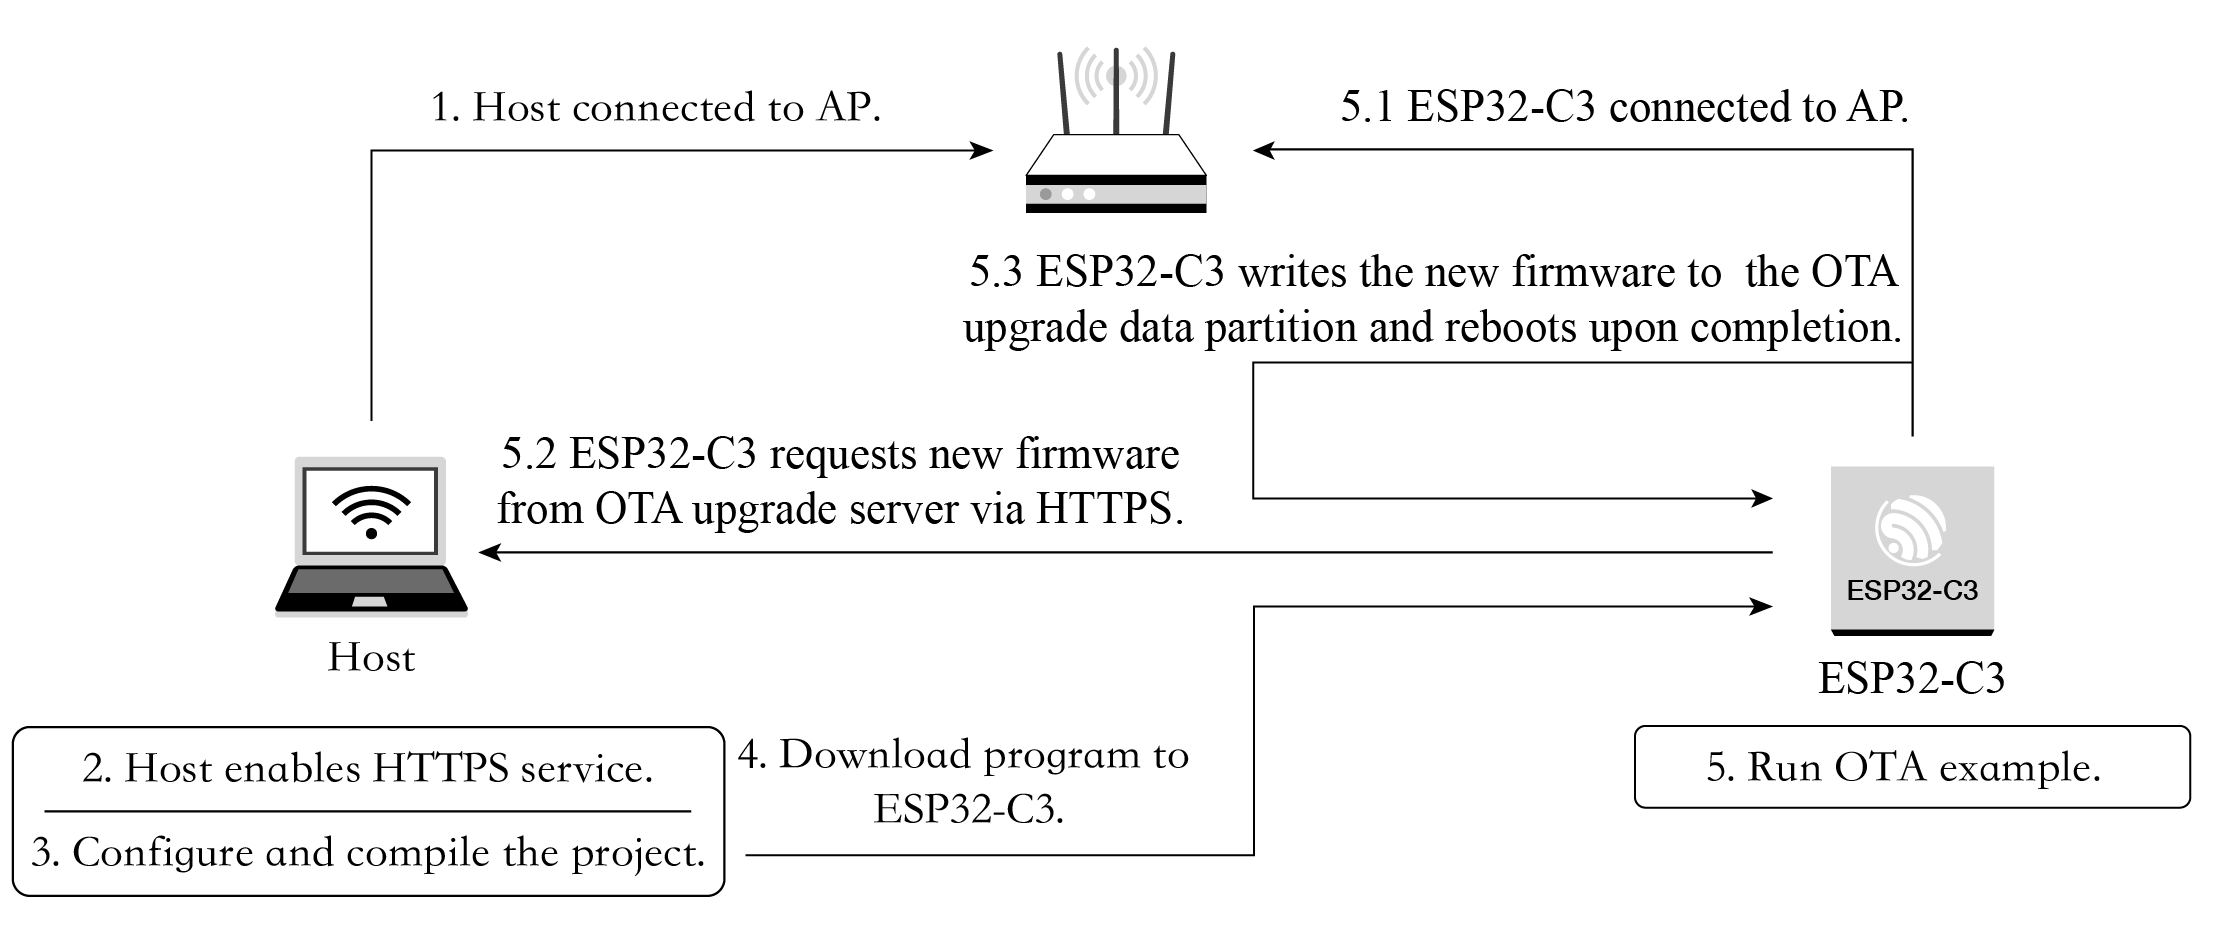
\includegraphics[width=0.8\textwidth]{D11Z/11-4}
    \caption{Procedure of over-the-air (OTA)}
\end{figure}

\textbf{(1) Enabling OTA server}

Before running the OTA example, you need to first create the HTTPS service and apply for a certificate. The certificate can be self-signed by executing \verb|openssl req -x509 -newkey|\\ \verb|rsa:2048 -keyout ca_key.pem -out ca_cert.pem -days 365 -nodes|. Logs are as follows:

\begin{codebloc}
\begin{tabular}{d}
\vspace{2pt}
\begin{verbatim}
Generating a RSA private key 
. +++++
....................+++++
writing new private key to 'ca_key.pem'
-----
You are about to be asked to enter information that will be incorporated
into your certificate request.
What you are about to enter is what is called a Distinguished Name or a DN.
There are quite a few fields but you can leave some blank
For some fields there will be a default value,
If you enter '.' , the field will be left blank.
-----
...
\end{verbatim}
\verb|...|
\end{tabular}
\end{codebloc}

\vspace{6pt}
\textbf{(2) Enabling HTTPS service}

The command \verb|openssl s_server -WWW -key ca_key.pem -cert ca_cert.pem |\\ \verb|-port 8070| will enable an HTTPS service with port 8070 on the local machine. The logs are as follows:

\begin{codebloc}
\begin{tabular}{d}
\vspace{2pt}
\begin{verbatim}
...
Using default temp DH parameters
ACCEPT
...
\end{verbatim}
\verb|...|
\end{tabular}
\end{codebloc}

Upon successful HTTPS connection, the logs are as follows:

\begin{codebloc}
\begin{tabular}{d}
\vspace{2pt}
\begin{verbatim}
139783954665920:error:14094416:SSL routines:ssl3_read_bytes:sslv3 alert 
certificate unknown:../ssl/record/rec_layer_s3.c:1528:SSL alert number 46
FILE:advanced_https_ota.bin
...
\end{verbatim}
\verb|...|
\end{tabular}
\end{codebloc}

\vspace{6pt}
\textbf{(3)	Using the \texttt{esp\_https\_ota} component to perform OTA}

Before the OTA test, let’s first look at how to write an OTA program. The following sample code comes from \href{https://github.com/espressif/esp-idf/blob/master/examples/system/ota/advanced_https_ota/main/advanced_https_ota_example.c}{\texttt{esp-idf/examples/system/ota/advanced\_https\_ota/main/\\ advanced\_https\_ota\_example.c}}:

\begin{codebloc}
\begin{tabular}{d}
\vspace{2pt}
\begin{verbatim}
1.  void app_main(void)
2.  {
3.    //Initialize NVS
4.    esp_err_t err = nvs_flash_init();
5.    if (err == ESP_ERR_NVS_NO_FREE_PAGES || err ==
6.                                      ESP_ERR_NVS_NEW_VERSION_FOUND) {
7.      ESP_ERROR_CHECK(nvs_flash_erase());
8.      err = nvs_flash_init();
9.    }
10.     ESP_ERROR_CHECK( err );
11.
12.     ESP_ERROR_CHECK(esp_netif_init());
13.     ESP_ERROR_CHECK(esp_event_loop_create_default());
14.
15.     //Initialize connection
16.     ESP_ERROR_CHECK(example_connect());
17.
18.     //firmware verification
19.     const esp_partition_t *running = esp_ota_get_running_partition();
20.     esp_ota_img_states_t ota_state;
21.     if (esp_ota_get_state_partition(running, &ota_state) == ESP_OK) {
22.       if (ota_state == ESP_OTA_IMG_PENDING_VERIFY) {
23.         if (esp_ota_mark_app_valid_cancel_rollback() == ESP_OK) {
24.           ESP_LOGI(TAG, "App is valid, rollback cancelled successfully");
25.         } else {
26.           ESP_LOGE(TAG, "Failed to cancel rollback");
27.         }
28.       }
\end{verbatim}
\verb|29.     }|
\end{tabular}
\end{codebloc}


\begin{codebloc}
\begin{tabular}{d}
\vspace{2pt}
\begin{verbatim}
30.
31. #if CONFIG_EXAMPLE_CONNECT_WIFI
32.     //Set PS mode
33.     esp_wifi_set_ps(WIFI_PS_NONE);
34. #endif 
35.     //Create Over-the-air (OTA) task
36.     xTaskCreate(&advanced_ota_example_task, "advanced_ota_example_task",
37.                     1024 * 8, NULL, 5, NULL);
\end{verbatim}
\verb|38. }|
\end{tabular}
\end{codebloc}

The above code snippet demonstrates the following procedure:

\begin{enumerate}[label=\alph*.]
    \item Initialise NVS with the \verb|nvs_flash_init()| function, which is generally the first step in writing an ESP32-C3 application.
    \item Initialise the \verb|netif| layer and connect to Wi-Fi with the \verb|example_connect()| function. This function is generic and is realised in the \verb|protocol_examples_common| component. You can replace it with your own Wi-Fi connection function.
    \item If rollback is enabled, then you need to set the firmware status.
    \item (Optional) Set the PS mode to \verb|WIFI_PS_NONE| with the \verb|esp_wifi_set_ps()| function to disable the power saving mode and achieve maximum data throughput.
    \item Create an OTA task and complete the firmware receiving process in the task. For proceduce of \verb|advanced_ota_ example_task|, please refer to Section 11.1.3.
\end{enumerate}

With the basic understanding of the above example, we can now proceed to the OTA test. Please perform and complete the following actions successively:

(1) Set the target chip to ESP32-C3 with the following command:

\begin{codebloc}
\begin{tabular}{d}
\$ \textbf{idf.py set-target esp32c3}
\end{tabular}
\end{codebloc}

\vspace{6pt}
(2) Set Wi-Fi information.

Run \verb|idf.py menuconfig| and edit the Wi-Fi SSID and password as follows:

\begin{codebloc}
\begin{tabular}{d}
\vspace{2pt}
\begin{verbatim}
(Top) → Example Connection Configuration
    Espressif IoT Development Framework Configuration
[*] connect using WiFi interface
(Xiaomi_32BD) WiFi SSID
(12345678) WiFi Password
[ ] connect using Ethernet interface
[*] Obtain IPv6 address
\end{verbatim}
\verb|    Preferred IPv6 Type (Local Link Address)  --->|
\end{tabular}
\end{codebloc}

\vspace{6pt}
(3) Set OTA information.

Fill in \verb|Firmware Upgrade| URL and select skipping server certificate CN fieldcheck and firmware version check.

\begin{codebloc}
\begin{tabular}{d}
\vspace{2pt}
\begin{verbatim}
(https://192.168.31.177:8070/advanced_https_ota.bin) Firmware Upgrade URL
[*] Skip server certificate CN fieldcheck
[*] Skip firmware version check
\end{verbatim}
\verb|(5000) OTA Receive Timeout|
\end{tabular}
\end{codebloc}

\vspace{6pt}
(4) Build firmware with the command \verb|idf.py build|.

After building, extract \verb|advanced_https_ota.bin| under the \verb|build| directory to the directory of the HTTPS server, namely, the directory where the \verb|openssl s_server| operation is performed.

(5) Download firmware.

Run \verb|idf.py flash monitor| to download the firmware and open monitor.

Upon completion of all operations, ESP32-C3 will power up and connect to the set Wi-Fi and reboot after downloading the firmware from the set URL.

\subsection{Upgrade Firmware Through ESP RainMaker}
A more common solution is to update firmware through a cloud platform. In this section, we’ll introduce how to push update messages from cloud to the device with ESP RainMaker. ESP RainMaker uses \verb|esp_https_ota| component as well. With the code of OTA integrated in the ESP RainMaker SDK, you can enable OTA by merely calling the \verb|esp_rmaker_ota_enable()| function. Note that while ESP RainMaker provides two ways of OTA, you need to select receiving OTA messages using topics. By subscribing topics related to OTA, you can receive MQTT messages, parse out the URL of the firmware, and push the progress and final status of the current update through these topics. The code for the ESP RainMaker OTA is stored under the \href{https://github.com/espressif/esp-rainmaker/tree/master/components/esp_rainmaker/src/ota}{\texttt{esp-rainmaker/components/esp\_rain\\ maker/src/ota}} directory. The code related to firmware downloads is stored in the source file \verb|esp_rmaker_ota.c| under the same directory, as well as the following code:

\begin{codebloc}
\begin{tabular}{d}
\vspace{2pt}
\begin{verbatim}
1.  //ESP RainMaker OTA status
2.  char *esp_rmaker_ota_status_to_string(ota_status_t status)
3.  {
4.      switch (status) {
5.          case OTA_STATUS_IN_PROGRESS:
6.          return "in-progress";
7.          case OTA_STATUS_SUCCESS:
8.          return "success";
9.          case OTA_STATUS_FAILED:
10.             return "failed";
11.             case OTA_STATUS_DELAYED:
12.             return "delayed";
13.             default:
14.             return "invalid";
\end{verbatim}
\verb|15.         }|
\end{tabular}
\end{codebloc}

\begin{codebloc}
\begin{tabular}{d}
\vspace{2pt}
\begin{verbatim}
16.         return "invalid";
17. }
18.
19.esp_err_t esp_rmaker_ota_report_status(esp_rmaker_ota_handle_t ota_handle,
20.                                       ota_status_t status,
21.                                       char *additional_info)
22. {
23.     ……
24.     if (ota->type == OTA_USING_PARAMS) {
25.         err = esp_rmaker_ota_report_status_using_params(ota_handle, status,
26.                                             additional_info);
27.     } else if (ota->type == OTA_USING_TOPICS) {
28.         err = esp_rmaker_ota_report_status_using_topics(ota_handle, status,
29.                                             additional_info);
30.     }
31.     ……
\end{verbatim}
\verb|32. }|
\end{tabular}
\end{codebloc}

There are four OTA statuses in ESP RainMaker: firmware acquisition in progress (\verb|OTA_|\\ \verb|STATUS_IN_PROGRESS|), OTA succeeded (\verb|OTA_STATUS_SUCCESS|), OTA failed (\verb|OTA_|\\ \verb|STATUS_FAILED|), and delayed (\verb|OTA_STATUS_DELAYED|).

Firmware acquisition in progress corresponds to the status of downloading firmware, which should be reported to the cloud platform when the \verb|esp_https_ota_begin()| function is called, and the cloud platform will then update the icon correspondingly. OTA succeeded and OTA failed indicate the results of firmware download and verification. Delayed indicates that the device is currently not available to process the request, and the OTA status can later be updated through the \verb|esp_rmaker_ota_report_status()| function.

\begin{codebloc}
\begin{tabular}{d}
\vspace{2pt}
\begin{verbatim}
1.  //Firmware information verification
2.  static esp_err_t validate_image_header(esp_rmaker_ota_handle_t ota_handle,
3.                                         esp_app_desc_t *new_app_info)
4.  {
5.      if (new_app_info == NULL) {
6.          return ESP_ERR_INVALID_ARG;
7.      }
8.
9.      //Firmware status aquisition
10.     const esp_partition_t *running = esp_ota_get_running_partition();
11.     esp_app_desc_t running_app_info;
12.     if (esp_ota_get_partition_description(running, &running_app_info) ==
13.                                                     ESP_OK) {
14.      ESP_LOGD(TAG, "Running firmware version: %s",running_app_info.version);
15.     }
16.
17.     //Verify project version number
\end{verbatim}
\verb|18. #ifndef CONFIG_ESP_RMAKER_SKIP_VERSION_CHECK|
\end{tabular}
\end{codebloc}

\begin{codebloc}
\begin{tabular}{d}
\vspace{2pt}
\begin{verbatim}
19.     if (memcmp(new_app_info->version, running_app_info.version,
20.                sizeof(new_app_info->version)) == 0){
21.         ESP_LOGW(TAG, "Current running version is same as the new.
22.                 We will not continue the update." );
23.         esp_rmaker_ota_report_status(ota_handle, OTA_STATUS_FAILED,
24.                                       "Same version received");
25.         return ESP_FAIL;
26.     }
27. #endif
28.
29.     //Verify project name
30. #ifndef CONFIG_ESP_RMAKER_SKIP_PROJECT_NAME_CHECK
31.     if (memcmp(new_app_info->project_name, running_app_info.project_name,
32.                         sizeof(new_app_info->project_name)) ! =  0 ){
33.         ESP_LOGW(TAG, "OTA Image built for Project: %s. Expected: %s",
34.                 new_app_info->project_name, running_app_info.project_name);
35.         esp_rmaker_ota_report_status(ota_handle, OTA_STATUS_FAILED,
36.                                      "Project Name mismatch");
37.         return ESP_FAIL;
38.     }
39. #endif
40.
41.     return ESP_OK;
\end{verbatim}
\verb|42. }|
\end{tabular}
\end{codebloc}

ESP RainMaker manages firmware by verifying the project version number and the project name. Only when the new and old firmware of the same project name are verified to have different project version numbers, the firmware downloading will then be allowed to continue. Generally speaking, the project version number is generally incremented, which is more conducive for version control. By comparing project names, you can prevent any accidental pushing of other products’ firmware.

\begin{codebloc}
\begin{tabular}{d}
\vspace{2pt}
\begin{verbatim}
1.static esp_err_t esp_rmaker_ota_default_cb(esp_rmaker_ota_handle_t ota_handle,
2.                                           esp_rmaker_ota_data_t *ota_data)
3.  {
4.      ……
5.      //OTA http parameter configuration
6.      esp_err_t ota_finish_err = ESP_OK;
7.      esp_http_client_config_t config = {
8.          .url = ota_data->url,
9.          .cert_pem = ota_data->server_cert,
10.             .timeout_ms = 5000,
11.             .buffer_size = DEF_HTTP_RX_BUFFER_SIZE,
12.             .buffer_size_tx = buffer_size_tx
13.         };
14. #ifdef CONFIG_ESP_RMAKER_SKIP_COMMON_NAME_CHECK
\end{verbatim}
\verb|15.         config.skip_cert_common_name_check = true;|
\end{tabular}
\end{codebloc}

\begin{codebloc}
\begin{tabular}{d}
\vspace{2pt}
\begin{verbatim}
16. #endif
17.     ……
18.     //Report update status
19.     esp_rmaker_ota_report_status(ota_handle, OTA_STATUS_IN_PROGRESS,
20.                                      "Starting OTA Upgrade");
21.
22.     ...
23.     ...
24.     //Establish HTTPS connection and prepare to download firmware
25.     esp_err_t err = esp_https_ota_begin(&ota_config, &https_ota_handle);
26.     if (err ! = ESP_OK) {
27.         ESP_LOGE(TAG, "ESP HTTPS OTA Begin failed");
28.         esp_rmaker_ota_report_status(ota_handle, OTA_STATUS_FAILED,
29.                                      "ESP HTTPS OTA Begin failed");
30.         return ESP_FAIL;
31.     }
32.     ……
33.     //Aquire firmware information for verification
34.     esp_app_desc_t app_desc;
35.     err = esp_https_ota_get_img_desc(https_ota_handle, &app_desc);
36.     if (err ! = ESP_OK) {
37.         ESP_LOGE(TAG, "esp_https_ota_read_img_desc failed");
38.         esp_rmaker_ota_report_status(ota_handle, OTA_STATUS_FAILED,
39.                                      "Failed to read image decription");
40.         goto ota_end;
41.     }
42.     err = validate_image_header(ota_handle, &app_desc);
43.     if (err ! = ESP_OK) {
44.         ESP_LOGE(TAG, "image header verification failed");
45.         goto ota_end;
46.     }
47.
48.     esp_rmaker_ota_report_status(ota_handle, OTA_STATUS_IN_PROGRESS,
49.                                  "Downloading Firmware Image");
50.     int count = 0;
51.
52.     // Download firmware cyclically
53.     while (1) {
54.         err = esp_https_ota_perform(https_ota_handle);
55.         if (err ! = ESP_ERR_HTTPS_OTA_IN_PROGRESS) {
56.             break;
57.         }
58.     ……
59.     }
60.
61.     // Release HTTPS resource after downloading and start verification
\end{verbatim}
\verb|62.     ota_finish_err = esp_https_ota_finish(https_ota_handle);|
\end{tabular}
\end{codebloc}

\begin{codebloc}
\begin{tabular}{d}
\vspace{2pt}
\begin{verbatim}
63.     if ((err == ESP_OK) && (ota_finish_err == ESP_OK)) {
64.         //Report OTA succeeded status to cloud after successful verification
65.         ESP_LOGI(TAG, "OTA upgrade successful. Rebooting in %d seconds..." ,
66.                 OTA_REBOOT_TIMER_SEC);
67.         esp_rmaker_ota_report_status(ota_handle, OTA_STATUS_SUCCESS,
68.                                     "OTA Upgrade finished successfully");
69.         esp_rmaker_reboot(OTA_REBOOT_TIMER_SEC);
70.         return ESP_OK;
71.     } 
72.     ……
\end{verbatim}
\verb|73. }|
\end{tabular}
\end{codebloc}

The \verb|esp_rmaker_ota_default_cb()| function is the default OTA callback function in ESP RainMaker and will be called once an OTA message is received from the cloud. The procedure of this function is similar to that of the OTA example function introduced in Section 11.1.3. The difference is that the \verb|esp_rmaker_ota_default_cb()| function includes the reporting of OTA status, which will update the current OTA progress of the device to the cloud platform in time.

\begin{codebloc}
\begin{tabular}{d}
\vspace{2pt}
\begin{verbatim}
1.  esp_err_t esp_rmaker_ota_enable(esp_rmaker_ota_config_t *ota_config,
2.                                  esp_rmaker_ota_type_t type)
3.  {
4.//Acquire partition information and verify firmware vadility through callback
5.      const esp_partition_t *running = esp_ota_get_running_partition();
6.      esp_ota_img_states_t ota_state;
7.      if (esp_ota_get_state_partition(running, &ota_state) == ESP_OK) {
8.          if (ota_state == ESP_OTA_IMG_PENDING_VERIFY) {
9.              ESP_LOGI(TAG, "First Boot after an OTA");
10.             //Run diagnostic function
11.             bool diagnostic_is_ok = true;
12.             if (ota_config->ota_diag) {
13.                 diagnostic_is_ok = ota_config->ota_diag();
14.             }
15.             if (diagnostic_is_ok) {
16.                 ESP_LOGI(TAG, "Diagnostics completed successfully!
17.                         Continuing execution ..." );
18.                 esp_ota_mark_app_valid_cancel_rollback();
19.             } else {
20.                 ESP_LOGE(TAG, "Diagnostics failed! Start rollback to the
21.                          previous version ..." );
22.                 esp_ota_mark_app_invalid_rollback_and_reboot();
23.             }
24.         }
25.     }
26.
27.     // Over-the-air (OTA) task callback function
\end{verbatim}
\verb|28.     if (ota_config->ota_cb) {|
\end{tabular}
\end{codebloc}

\begin{codebloc}
\begin{tabular}{d}
\vspace{2pt}
\begin{verbatim}
29.         ota->ota_cb = ota_config->ota_cb;
30.     } else {
31.         ota->ota_cb = esp_rmaker_ota_default_cb;
32.     }
33.     ……
34.     return err;
\end{verbatim}
\verb|35. }|
\end{tabular}
\end{codebloc}

The OTA part in ESP RainMaker encapsulates the self-test segment of the rollback function. You can input a self-test function with a Boolean return value through the \verb|esp_rmaker_ota|\\ \verb|_config_t| structure. When calling the \verb|esp_rmaker_ota_enable()| function to enable OTA, once the current firmware status is found to be pending for verification (\verb|ESP_OTA_IMG_|\\ \verb|PENDING_VERIFY|), the self-test function input previously will be called by the function pointer, and the current firmware status will be set through the return value of the self-test function. \verb|server_cert| in the \verb|esp_rmaker_ota_config_t| structure points to the server-side certificate. ESP RainMaker uses AWS S3 bucket storage service, and you can pass in the certificate directly via the macro \verb|ESP_RMAKER_OTA_DEFAULT_SERVER_CERT|, which is used during OTA to perform verifications and prevent DNS spoofing. You can upload the new firmware in the management backend of ESP RainMaker. The project version of the new firmware must be different from the version expected to be updated to, and there are two ways to modify the version in ESP RainMaker:

\begin{enumerate}[label=(\arabic*)]
    \item Modify the project version number introduced in Section 11.2.1.
    \item Modify the \verb|CMakeLists.txt| file by adding \verb|set(PROJECT_VER "1.0")|. You may refer to the example about this part.
\end{enumerate}

Once the new firmware is built, you can upload the new firmware as shown in Figure 11.5.

\begin{figure}[h!]
    \centering
    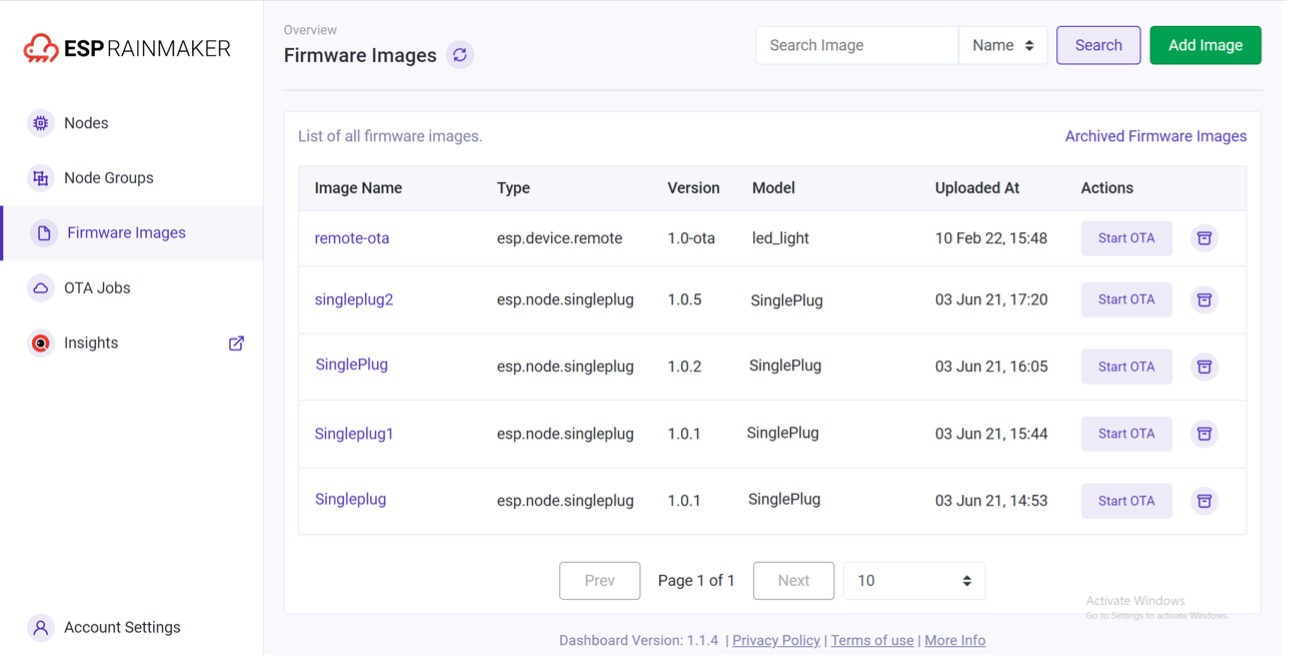
\includegraphics[width=0.85\textwidth,frame]{D11Z/11-5}
    \caption{Uploading new firmware}
\end{figure}

Once the firmware is uploaded, you can enable the OTA task as shown in Figure 11.6. The procedure of booting the OTA task is as follows:

\begin{figure}[h!]
    \centering
    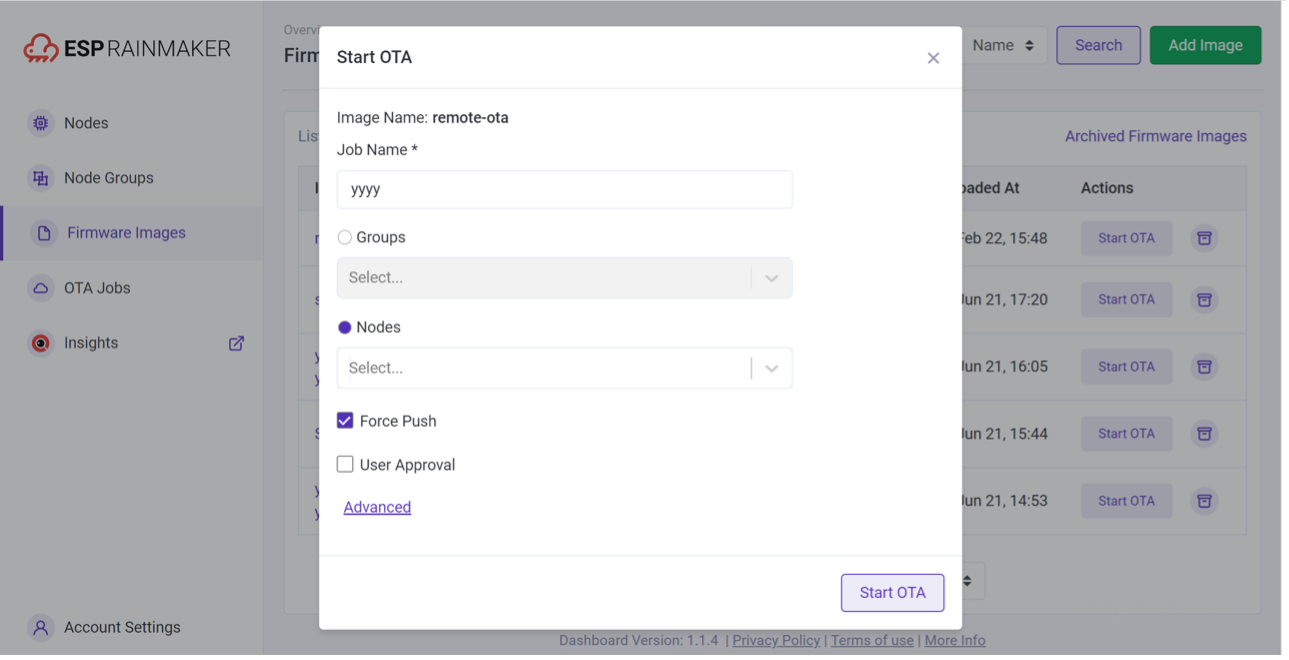
\includegraphics[width=0.85\textwidth]{D11Z/11-6}
    \caption{Boot the OTA task}
\end{figure}

\begin{enumerate}[label=(\arabic*)]
    \item Select the firmware used for OTA from the list.
    \item Click “Start OTA” for the firmware.
    \item Fill in information of the OTA task and select the node to be updated. When the “Force Push” option is selected, online nodes can receive OTA messages immediately. Otherwise, nodes will obtain URLs for OTA based on the defined OTA policy (checks during startup, periodic checks, etc.), which may cause delays.
\end{enumerate}

\begin{figure}[h!]
    \centering
    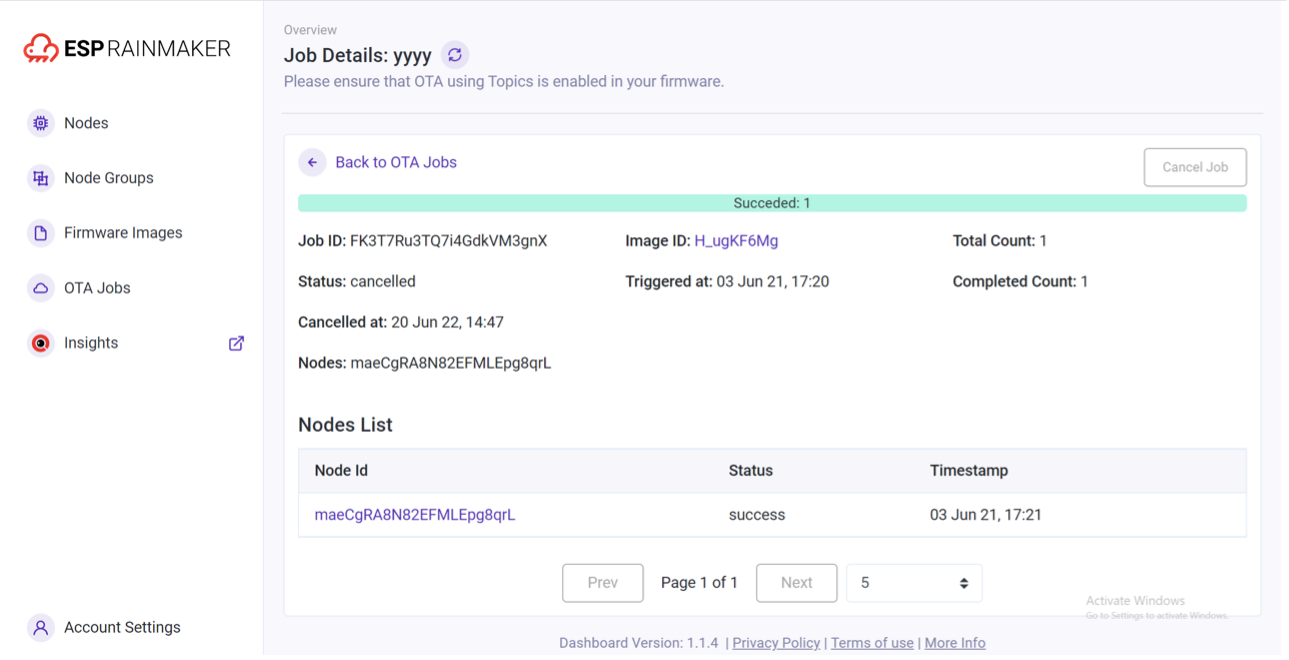
\includegraphics[width=0.85\textwidth,frame]{D11Z/11-7}
    \caption{ Interface of OTA Job Monitor}
\end{figure}

The OTA Job Monitor (see Figure 11.7) provides real-time feedback on the status of OTA, including the information available to users and the functions implemented.

\begin{itemize}
    \item After initiating OTA successfully, the OTA status can be checked in the task details of the current OTA job, which are reported by the device.
    \item The OTA Job Monitor will provide an overview of the task and the status of each node can be checked.
    \item The OTA task can be cancelled midway, but the nodes which have already obtained the URL will continue upgrading.
\end{itemize}

\section{Summary}
This chapter mainly introduces the mechanism and procedures of OTA. Firstly, it describes the basic procedures and ways of performing OTA. Then it presents the functions of the partition table and the fields related to OTA. In actual mass production, it is also necessary to enable the rollback and anti-rollback functions accordingly to further improve the stability and reliability of the device. Finally, according to the practical example provided, you can either complete the firmware update through the local host or push the update message to the device from the cloud through ESP RainMaker.

\end{document}